\documentclass[thesis-solanki.tex]{subfiles}



\ifMain
\externaldocument{thesis-solanki}
\fi
\begin{document}

% ---------------------------------------------------------------------------
\chapter{\progLang{Prolog}}\label{chap:pwp}
% ---------------------------------------------------------------------------
%Prolog / Why Prolog ?


\section{About this chapter}

This chapter discusses the properties of the target language \progLang{Prolog} and the feature set that will be translated to the host 
language to extend its capabilities.
\progLang{Prolog} is a general purpose logic programming language mainly used in artificial intelligence and
  computational linguistics.
  It is a declarative language, i.e., a program is a set of facts an rules running a
  query on which will return a result.
  The relation between them is defined by clauses using \textit{Horn Clauses} \cite{wikiprolog}.
  \progLang{Prolog} is very popular and has a number of implementations
  \cite{website:comparisonofprologimplementationswiki} for different purposes.
  
\section{Logic programming language}

%Our base language, \progLang{Haskell}, is from the same paradigm. It would be interesting to see how two languages of the same family with 
%conflicting features can be made to work together.

One of the reasons is that both \progLang{Haskell}, the base language and \progLang{Prolog}, the target language are from the same paradigm.
This provides a platform to play around with the conflicting characteristics of the two languages.


\section{Simple Syntax}

\progLang{Prolog} is dynamically typed. It has a single data type, the term, which has several subtypes: atoms, numbers, variables and 
compound terms \cite{wikiprolog}.


An atom is a general-purpose name with no inherent meaning. It is composed of a sequence of characters that is parsed by the 
\progLang{Prolog} reader as a single unit.

Numbers can be floats or integers. Many \progLang{Prolog} implementations also provide unbounded integers and rational numbers.

Variables are denoted by a string consisting of letters, numbers and underscore characters, and beginning with an upper-case letter or 
underscore. Variables closely resemble variables in logic in that they are placeholders for arbitrary terms. A variable can become 
instantiated (bound to equal a specific term) via unification.

A compound term is composed of an atom called a ``functor'' and a number of ``arguments'', which are again terms. Compound terms are 
ordinarily written as a functor followed by a comma-separated list of argument terms, which is contained in parentheses. The number of 
arguments is called the term's arity. An atom can be regarded as a compound term with arity zero.


A \progLang{Prolog} program is a description of relations, defined by the use of clauses. Pure \progLang{Prolog} is restricted to Horn 
clauses, a Turing-complete subset of first-order predicate logic. The clauses can be one of two types: facts and rules 
\cite{website:prologintroumiami}.

\begin{comment}
In \progLang{Prolog}
 all data objects are called terms.\endnote{%
   Fix.
}
 Atomic terms
 come in two forms: atoms and integers.
 Atoms (this is a misnomer,\endnote{%
   Fix
}
 as in logic predicates are called atoms, and atoms are called constants. However, we'll stick to the 
 \progLang{Prolog}\endnote{%
   Fix.
}
 convention.)
consist of
strings of alphanumerics and ``\texttt{\_}'', starting with a lower case alphabetic.
Strings enclosed in 'single quotes'\endnote{%
  What?
}
Integers are numeric.
Example
\par
\begin{minted}[linenos]{prolog}
geoff
'the cat and the rat'
'ABCD'
123
\end{minted}
\end{comment}

\begin{comment}
\subsection{Function terms}

Functions have the form \Verb!<functor>(<term>{,<term>})!
where \Verb!functor! starts with a lower-case alphabetic. 
\paragraph{Example}
\par
\begin{minted}[linenos]{prolog}
prerequisite_to(adv_ai)
grade_attained_in(prerequisite_to(adv_ai),pass)
\end{minted}
     
The number of arguments is the arity of the function. When referring to a functor, it is written with its arity in
the format \Verb!<functor>/<arity>!. This is also true for atoms, whose arity is 0.
Note that this is a recursive definition.
\paragraph{The view of functions as trees}
\subparagraph{Operators}
Some functors are used in infix notation, e.g., \Verb!5+4!.
Operators do not cause the associated function to be carried out.
\subparagraph{Variables}

Uppercase or `\Verb!_!' start variables.
\paragraph{Example}
\begin{minted}[linenos]{prolog}
Who
What
_special
_
\end{minted}
     
Variables in \progLang{Prolog} are rather different from those in most other languages. Further discussion and use is deferred until later.

\end{comment}

\section{Simple Semantics}

Since the commutative nature of logical disjunction and conjunction, declaratively speaking the order of rules and their sub goals is
irrelevant. However, the procedural aspect must be taken into account to determine the execution strategy of \progLang{Prolog} since it
has to deal with impure predicates. Moreover, a particular order of execution can lead to infinite recursion.

\section{Universal Horn clauses}


\section{Unification}



\section{Definite clause grammar}

\section{How \progLang{Prolog} works}

To replicate \progLang{Prolog} we look into how it works \enparen{see, for instance,
      \textup{\cite{webiste:learnprolognow}}}.
%
As any other language we start with the syntax and semantics.
We begin with the programming constructs of the language.

\progLang{Prolog} has three types of terms: constants, variables and complex terms.

Two terms can be unified if they are the same or the variables can be assigned to terms such that the resulting
terms are equal.

The possibilities are:
\begin{enumerate}
\item If \mSV{term1} and \mSV{term2} are constants, then \mSV{term1} and \mSV{term2} unify if and only if they
  are the same atom, or the same number. Consider the example in Listing~\ref{tab:unifyingconstants}
\par
\begin{code-list}[H]
\begin{singlespace}
\inputminted{prolog}{prolog-pwp-unify-constants.pl}
\end{singlespace}
\caption{Unification with constants.}
\label{tab:unifyingconstants}
\end{code-list}


\item If \mSV{term1} is an uninstantiated variable and \mSV{term2} is any type of term, then \mSV{term1}
  and \mSV{term2} unify, and \mSV{term1} is instantiated to \mSV{term2}\,.
  Similarly, if \mSV{term2} is a variable and \mSV{term1} is any type of term, then \mSV{term1} and \mSV{term2}
  unify, and \mSV{term2} is instantiated to \mSV{term1}.
  Consider the examples in Listing~\ref{tab:unificationsinglevariable} and 
  Listing~\ref{tab:unificationmultiplevariable}. (So if they are both 
variables, they're both instantiated to each other, and we say that they share values.)
\par
\begin{code-list}[H]
\begin{singlespace}
\inputminted{prolog}{prolog-pwp-unify-single-variable.pl}
\end{singlespace}
\caption{Unification with a single variable.}
\label{tab:unificationsinglevariable}
\end{code-list}

\begin{code-list}[H]
\begin{singlespace}
\inputminted{prolog}{prolog-pwp-unify-multi-variable.pl}
\end{singlespace}
\caption{Unification with variables.}
\label{tab:unificationmultiplevariable}
\end{code-list}




\item If \mSV{term1} and \mSV{term2} are complex terms, then they unify if and only if:

\begin{enumerate}
\item they have the same functor and arity, and

\item all their corresponding arguments unify, and

\item the variable instantiations are compatible.
\end{enumerate}
Consider the example in Listing~\ref{tab:unificationcomplexterms}.
\par
\begin{code-list}[H]
\begin{singlespace}
\inputminted{prolog}{prolog-pwp-unify-complex-terms.pl}
\end{singlespace}
\caption{Unification of complex terms.}
\label{tab:unificationcomplexterms}
\end{code-list}



\item Two terms unify if and only if it follows from the previous three clauses that they unify.
\end{enumerate}

Unification is just a part of the process where the language
attempts to find a solution for the given query using the rules provided
in the knowledge base.
The other part (searching) is to reach a point where two terms are required to be unified.
Together they form the query resolver in \progLang{Prolog}.

For example, consider the append function shown in Listing~\ref{tab:prlgappnd}.

\begin{code-list}[H]
\begin{singlespace}
\inputminted{prolog}{prolog-pwp-append.pl}
\end{singlespace}
\caption{append function in \progLang{Prolog}}
\label{tab:prlgappnd}
\end{code-list}
%
whose operation is illustrated in Figure~\ref{fig:Trace for append}.

\begin{figure}[H]
\centering
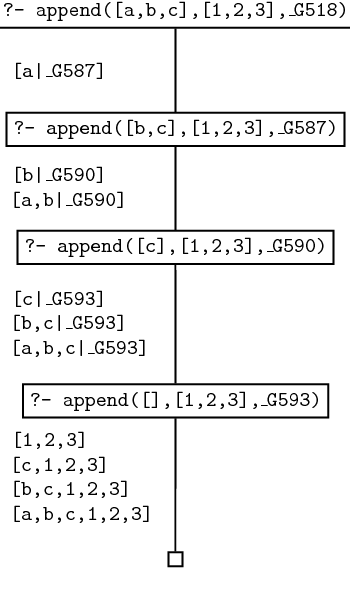
\includegraphics[scale = 0.5]{PrologAppendWorking.png}
\caption{Trace for append \cite{webiste:learnprolognowappend}}
\label{fig:Trace for append}
\end{figure}


\section[{The execution models of \progLang{Prolog}}]{The execution models of \progLang{Prolog} \cite{Sterling:1994:APA:175753}\endnote{
\david{Move the citation from the section title, and explicitly state that
  the material here has been exerpted from
  \cite{Sterling:1994:APA:175753}, with page or chapter references.
}
\mehul{changed}
}
}\label{sec:exec-models-prolog}
Logic programming languages are adapted from abstract interpreters for logic programs. 
To implement a logic programming language such as \progLang{Prolog} two major decisions must be taken to resolve a query\endnote{
\david{Rewrite this to be clear about the differences between an
  \textit{abstract} \progLang{Prolog} and the choices made by concrete
  implementations, such as Edinburgh \progLang{Prolog}.
}
\mehul{changed}
}:
\begin{enumerate}
\item Scheduling policy:
Select leftmost goal and replace the non deterministic choice of a clause by sequential search for a unifiable clause and backtracking. 
Stack scheduling policy, pop the topmost goal for reduction and push derived goals back.

\item Search strategy:
\progLang{Prolog} simulates the non-deterministic choice of reducing clause by sequential search and backtracking. The first goal whose 
head unifies with the goal is chosen. If no match is found then the computation is unwound to the last choice point and the next unifiable 
clause is chosen.
\end{enumerate}

\progLang{Prolog} generates all possible solutions of the goal with respect to the \progLang{Prolog} program. It performs a complete
depth first traversal of a particular search tree for the goal by always choosing the leftmost goal. Listing~\ref{tab:prlgprgrmtrce} shows
a sample trace for a query.

\begin{code-list}[H]
  \begin{singlespace}
    \inputminted[linenos]{prolog}{prologprogramtrace.pl}
  \end{singlespace}
  \caption{Tracing a simple Prolog computation \cite{Sterling:1994:APA:175753}}
\label{tab:prlgprgrmtrce}
\end{code-list}

As seen in Listing~\ref{tab:prlgprgrmtrce} how \progLang{Prolog} resolves a query. Consider the example in 
Listing~\ref{tab:prlgcutfreeexmpl}. A sample query \prologConstruct{p(X)} will result in \ref{tab:prlgcutfreeexmploutput}. 

\begin{code-list}[H]
  \begin{singlespace}
    \inputminted[linenos]{prolog}{prlgcutfreeexmpl.pl}
  \end{singlespace}
  \caption{A cut-free Prolog computation \cite{website:cutprologunionedu}}
\label{tab:prlgcutfreeexmpl}
\end{code-list}

\begin{code-list}[H]
  \begin{singlespace}
    \inputminted[linenos]{prolog}{prlgcutfreeexmploutput.pl}
  \end{singlespace}
  \caption{cut-free Prolog computation output\cite{website:cutprologunionedu}}
\label{tab:prlgcutfreeexmploutput}
\end{code-list}

A \prologConstruct{cut} represented as \prologConstruct{!} operator \cite{website:prologcut}.
If \progLang{Prolog} finds a \prologConstruct{cut} in a rule, it will not backtrack on the choices it has made. Consider the example below:

\mint{prolog}|p(X) :- b(X),c(X),!,d(X),e(X).|

The result for a sample query \prologConstruct{p(X)}:
\mint{prolog}|X = 1 ; no|

Only a single solution is obtained because the \prologConstruct{cut} prevents backtracking. The Figure~\ref{fig:Trace with cut} shows the 
trace for the query with the \prologConstruct{cut} operator.

\begin{figure}[H]
\centering
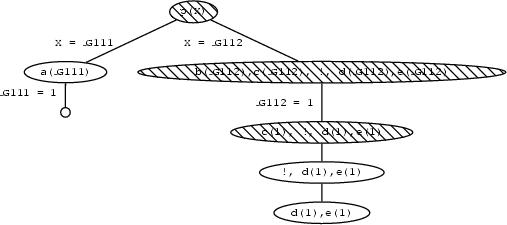
\includegraphics[scale = .95]{prologcutrace.jpeg}
\caption{Trace with cut (taken from \cite{website:cutprologunionedu})}
\label{fig:Trace with cut}
\end{figure}


\endnote{
  \david{say something about cut here}
\mehul{changed}
}


\section{Embedding \progLang{Prolog}}

\begin{comment}
Existing implementations

As a starting point a few publications and implementations helped in exploring the topic. The shortcomings were clearly visible to work and
improve upon giving a starting point.
\end{comment}

\progLang{Prolog} seems to be a very popular choice as a target language. Also for the specific topic of embedding \progLang{Prolog} in 
\progLang{Haskell}, implementations and publications exist which provide a starting point.\endnote{%
  The surrounding \macroName{begin}\macroArg{enumerate} should be a
  \texttt{description} environment, or a list of
  \macroName{sub}\textsuperscript{\textasteriskcentered}\texttt{section}'s.
	\mehul{changed}
}


\section{Chapter recapitulation}
Recapitulating, this chapter provided information on \progLang{Prolog} as a logic programming language.

\ifMain
\begin{scope}
  \nolinenumbers
  \enotesize
  \par
  \begin{singlespace}
  \setlength{\parskip}{12pt plus 2pt minus 1pt}
  \theendnotes
  \par
  \end{singlespace}
\end{scope}
\unbcbibliography{bibliography}
\fi

\end{document}
